\documentclass[11pt]{article}

\usepackage[utf8]{inputenc}
\usepackage[english]{babel}

\usepackage{mathtools}

\usepackage{setspace}
\onehalfspacing

\usepackage{amsfonts}
\usepackage{amsmath}
\usepackage{amsthm}
\usepackage{indentfirst}
\newtheorem{theorem}{Theorem}
\newtheorem{lemma}{Lemma}
\newtheorem{example}{Example}
\newtheorem{definition}{Definition}
\newtheorem{remark}{Remark}
\newtheorem{corollary}{Corollary}

\newtheorem*{theorem*}{Theorem}
\newtheorem*{lemma*}{Lemma}
\newtheorem*{example*}{Example}
\newtheorem*{definition*}{Definition}
\newtheorem*{remark*}{Remark}
\newtheorem*{corollary*}{Corollary}

%\usepackage{booktabs, caption, graphicx, float}
%\usepackage{subcaption}
%\captionsetup{tableposition=top,figureposition=bottom,font=small}

\usepackage{comment}
\usepackage{multirow}
\usepackage{array}

\newcolumntype{C}[1]{>{\centering\let\newline\\\arraybackslash\hspace{0pt}}m{#1}}
\DeclarePairedDelimiter\floor{\lfloor}{\rfloor}

\usepackage[hidelinks]{hyperref}

\usepackage{geometry}
\geometry{a4paper, top=3cm,bottom=3cm,left=3cm,right=3cm,%
	heightrounded}
\usepackage{upgreek}
\usepackage{xparse}
\usepackage{listings}
\NewDocumentCommand{\codeword}{v}{%
	\texttt{\textcolor{black}{#1}}%
}

\newcommand{\prepos}[3]{${}_{\mathbf{#2}}{\mathbf{#1}}_{#3}$}
\newcommand{\preposm}[3]{{}_{\mathbf{#2}}{\mathbf{#1}}_{#3}}


%Dummy text
\usepackage{lipsum}

%Changing headers and footers
\usepackage{fancyhdr}
\pagestyle{fancy}
\fancyhf{}
\rhead{\textit{\thepage}}
\lhead{\textit{ Task Space Motion Control Lab}}

%For inserting the code
\usepackage{fancyvrb}

%For bold math symbols
\usepackage{bm}

%For multicolumns
\usepackage{multicol}

% Norm and abs delimiter
\usepackage{mathtools}
\DeclarePairedDelimiter{\abs}{\lvert}{\rvert}
\DeclarePairedDelimiterX{\norm}[1]{\lVert}{\rVert}{#1}

\setcounter{section}{-1}

% Argmin/Argmax
\DeclareMathOperator*{\argmax}{argmax}
\DeclareMathOperator*{\argmin}{argmin}

% Enumerate
\usepackage{enumitem}

% Code
\usepackage{algorithm}
\usepackage[noend]{algpseudocode}
\usepackage{etoolbox}

% Longtable
\usepackage{longtable}

% SI units
\usepackage{siunitx}
\sisetup{output-exponent-marker=\ensuremath{\mathrm{e}}}

% Colours in equations
\usepackage{xcolor}

\newcommand{\Rnum}{\mathbb{R}} % Symbol fo the real numbers set
\newcommand{\mat}[1]{\ensuremath{\begin{bmatrix}#1\end{bmatrix}}}	% matrix
\newcommand{\myparagraph}[1]{\paragraph{#1}\mbox{}\\}


\title{LAB 7: Admittance Control}
\author{Michele Focchi and Matteo Saveriano}
\date{}

\begin{document}
	\maketitle
	\noindent
	The goals of this assignment are:
	\begin{itemize}
		\item learning the basic procedure to design an admittance controller for the end-effector of a manipulator in contact with the environment with the purpose to control the interaction
		\item Implement a postural task to solve the indeterminacy when performing inverse kinematics. 
	\end{itemize}
	
	\noindent
	Tools that we are going to be using in this lab (all open-source):
	\begin{itemize}
		\item Python programming (2.7)\footnote{https://docs.python.org/2.7/}
		\item Robot Operating System (ROS)\footnote{https://www.ros.org/}
		\item Gazebo \footnote{http://gazebosim.org/}
		\item Pinocchio Library for Rigid Body Dynamics Algorithms\footnote{https://github.com/stack-of-tasks/pinocchio}
		\item Locosim\footnote{https://github.com/mfocchi/locosim}
	\end{itemize}
	%
	%
	%\noindent
	In this assignment we will modify the set-point for the end-effector computed in previous labs, using an admittance model, to accommodate for an external force acting at the end-effector. An inverse kinematics scheme will map the corrected references to joint space where we will close the loop for tracking. The implementation of and admittance scheme might be the only way to be able to  achieve safe interactions with industrial robots. This is because, most of the times, industrial robot are not equipped with an inner torque loop, but with a (stiff) position one plus a 6 axis force sensor located at the end-effector. Differently from the approaches seen until now that enable a safe interaction with any part of the robot, this approach allows  
	the robot to be compliant (and safe) \textit{only} if the interaction occurs at the end-effector location, where we are able to 
	sense the force. 
	
\section{Preliminaries}
	The robot that we will use this time, is still the  Ur5 robot, but, differently from before, we will not integrate the dynamics ourself but this will be done by a simulator called Gazebo. An intermediate controller ( \codeword{ros_impedance_controller}) will receive the PD gains and the set-point of desired joint positions and velocities and feed-forward torques from our Python node, this controller will either interface to the simulator Gazebo or to the real robot. This has the big advantage of  allowing us to use the same code in both situations.

\section{Admittance Control}
An admittance control framework requires two components: an \textit{admittance model} and an \textit{inverse kinematics} function.
The philosophy behind admittance control is to change the end-effector position set-point in order to mimic a desired admittance at the end-effector. We recall that an admittance is a linear model that receives  as input a \textit{force} and outputs a displacement $\Delta p_e$ (or a velocity). Then, the displacement $\Delta p_e$ is added to the set-point creating a new reference for the end-effector $\tilde{p_e}^d = \Delta p_e + {p_e}^d$  that is mapped to joints references via an inverse kinematics function, as shown in figure \ref{fig:admittance}:

\begin{figure}[bht]
	\centering
	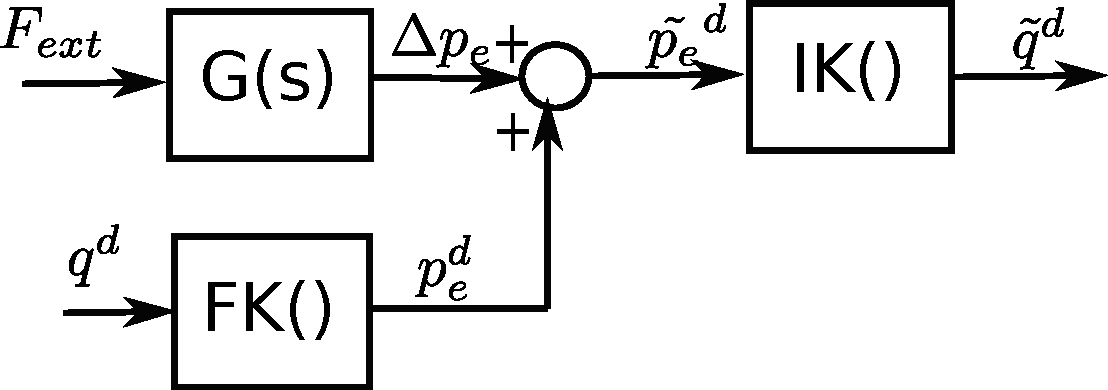
\includegraphics[width=8cm]{admittanceControl.pdf}
	\caption{Block diagram for an admittance controller in the Cartesian space. FK(.) and IK(.) are the forward and inverse kinematics blocks, respectively, while G(s) is the admittance model.}
	\label{fig:admittance}
\end{figure}

\quad

\noindent
\textbf{1.1 - Implement the admittance model }\\
We want to implement an admittance model that represents a \textit{linear} virtual spring and a \textit{linear} virtual damper at the end-effector.
The transfer function G(s) for this model in the Laplace domain is :



\begin{align}
\label{eq:tf}
\Delta p_e &= \frac{ F_{ext} }{K_d s + K_p}\\
G(s)& = \frac{\Delta p}{F_{ext}} = \frac{ 1 }{K_d s + K_p} \nonumber
\end{align}


Where the input is the contact force $F_{ext}\in \Rnum^3$ and the output the shift  $\Delta p_e\in \Rnum^3$ to be applied to the end-effector reference to emulate a virtual stiffness in response to  $F_{ext}$. Note that this transfer function is in continuous time and we need a discretized version for a digital implementation on a computer. To get the discrete version, it is convenient to convert \eqref{eq:tf} first in the time domain:

\begin{align*}
K_d \Delta\dot{ p_e} + K_p{\Delta p_e}  =  F_{ext}  
\end{align*}
 
Then, if  we  employ Forward Euler $\dot{p_e} = (p_e(k)- p_e(k-1))dT^{-1}$ to approximate the derivative, we can get the following difference equation:

\begin{align*}
&K_d \frac{p_e(k)- p_e(k-1)}{dT}  + K_p \Delta p_e(k)  =  F_{ext}(k)  \\
&\Delta p_e(k) (K_d dT^{-1} + K_p ) - K_d \Delta p_e(k-1)dT^{-1} =  F_{ext}(k)\\
&\Delta p_e(k) =  (K_d dT^{-1} + K_p )^{-1} (F_{ext}(k) + K_d \Delta p_e(k-1)dT^{-1})
\end{align*}

where (k)and (k-1) refer to the actual and previous samples of the variables. 


\quad

\noindent
\textbf{1.2 - Inverse Kinematics}\\
Now that we wrote a function to implement the admittance model, we still miss to implement the inverse kinematics function. To be able to convert the modified reference $\tilde{p_e}^d(k) = p_e^d(k) +  \Delta p_e(k)$  at each loop $k$ into a joint reference $q^d$. Note that, since our admittance model (composed of linear spring and damper)  involves only 3D vectors, and we have 6 DoFs in our robot, we will have redundancy, hence  infinite solutions to the inverse kinematics problem. 
To solve this issue we can implement a ``postural task'' at the kinematic level to solve the redundancy.
This will  selects among the infinite solutions the one (joint configuration $\tilde{q}^d$) that is closer (in an Euclidean sense) to a desired configuration (e.g. the initial one). In this manner we avoid that the robot jumps randomly from a configuration to another.) 
To obtain this, we setup the following optimization problem:

\begin{align*}
\tilde{q}^d = \argmin_q \frac{1}{2} \left|\left| \mat{p(q) \\ w q } - \mat{p^d \\ w q^p }   \right|\right|^2 = \frac{1}{2} \left|\left| \mat{ e_x \\ e_q }   \right|\right|^2
\end{align*}

where $w$ is a scalar weight and $q^p$ the postural configuration. The solution of this optimization problem (which is non convex do to the non linear dependency of $p_e$ from $q$) can be obtained through the Newton method, in a similar fashion to what we did in lab L1 - 2.4. The difference is the definition of the error $\bar{e} = \mat{e_x^T & e_q^T}^T$ (than now will be a 6D vector) and the way the newton step $\Delta q$ is computed:


\begin{align*}
\Delta q &= -\left( \mat { J^T &  wI_{3 \times 3} } \underbrace{ \mat{J  \\ wI_{3 \times 3}}}_{\bar{J}} \right)^{-1} \left(J^T e_x + w^2e_q \right) \\
	    &= -\left( J^TJ + w^2I_{3 \times 3}\right)^{-1} \underbrace{ \left(J^T e_x + w^2 e_q \right) }_{\bar{J}^T\bar{e}}
\end{align*}

note that we have a minus sign just because we defined differently $e_p$ (in L1 -2.4 we were using $e_p = p^d- p$ instead of $e_p = p - p^d$). So, with respect to the L1 -2.4: 1) we use $w^2$ instead of $\lambda $ to regularize, 2) we added ad term $w^2 e_q $ to the gradient, 3) we changed the stopping criteria of the IK algorithm by checking if the norm of this new gradient $\bar{J}^T\bar{e}$ goes below $\epsilon$.


\quad

\noindent
\textbf{1.3 - External push with a constant reference}\\
Now we are ready to test the implemented algorithm. Set  a constant joint reference $q_0$  for the robot to follow (that will correspond to a constant end-effector position) and set the admittance gains to $K_p = 1000I_{3\times3}$,  $K_d = 300I_{3\times3}$. We can how the controller works by applying an external force either in simulation (calling the function \codeword{applyForce()} after 5 seconds) or pushing manually (gently!) the end-effector (Important! keep always the E-stop in your hand to kill the robot in case some instability arise!). You should feel the robot deviating from the reference in the same direction of the force (we are setting a diagonal stiffness matrix), as if a spring is attached at the end-effector trying to push it back to the original position. 
Now try to reduce the stiffness gain to $K_p = 600I_{3\times3}$, in order to make the robot more ``soft''. You should feel that for the same force you are applying you are getting a bigger deflection (almost double).
Plot the signals of the end-effector position and force to evaluate the direction of the deflection is consistent with the force.

\textbf{1.3 - External push with a sinusoidal reference}
Let's now apply a sinusoidal reference to the robot joints  with amplitude $A= 0.1$ $rad$ and frequency $f = 0.2$ $Hz$, around the initial position $q_0$.

\begin{align*}
q^d(t) = q_0 + Asin(2\pi f t )
\end{align*} 

Now, apply the external disturbance, \textit{while} the robot is moving. You should see the end-effector deviating from the original trajectory in the direction of the pushing force. 
 
\end{document}